\clearpage
\section{Auswertung}

\subsection{Messungen bis 1 Bar}

\subsubsection{Plot der Messwerte und Funktionen}
Im folgenden Plot sind die Messwerte und die dazugehörige berechnete Fit-Funktion \refeq{eqn:fit1} zusehen.
Hier wurde der Logarithmus des Drucks gegen den Kehrwert der Temperatur aufgetragen.
Dies dient zur Bestimmung von $L$ in der Theorie 
bereits dargestellten Zusammenhang \refeq{eqn:steigung}.
\begin{figure}[htp]
    \centering
    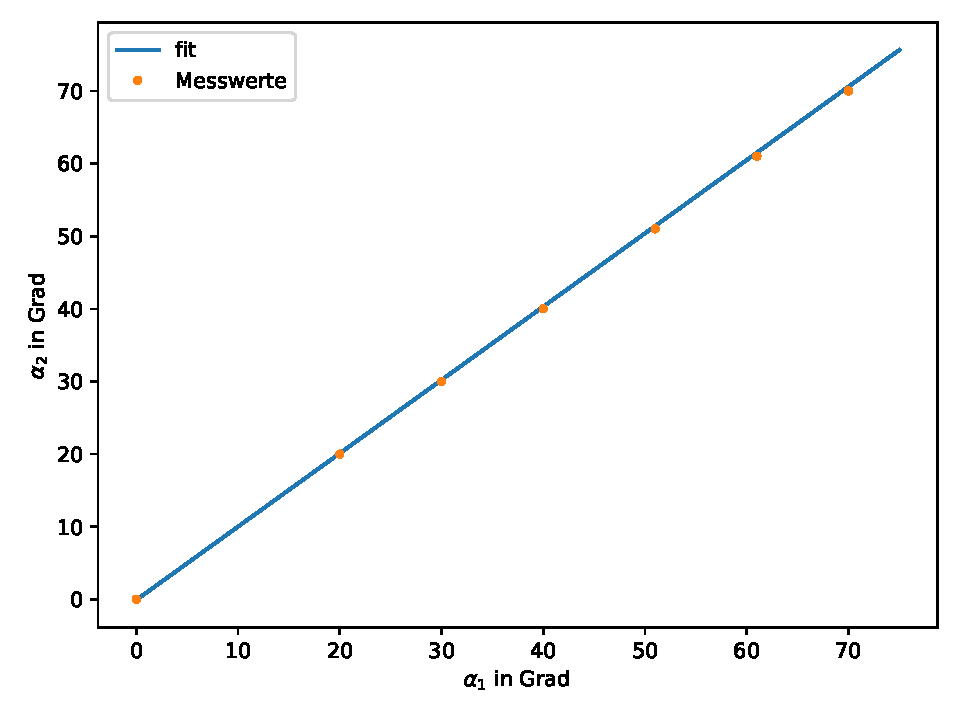
\includegraphics[width=0.7\textwidth]{build/plot1.pdf}
    \caption{Ein Plot der Messwerte inklusive der gefiteten Funktionen.}
    \label{img:plot1}
\end{figure}
\FloatBarrier


\subsubsection{Berechnung von L}

Die gefittete Funktion auf die Messwerte \ref{tab:messung1} wurde mithilfe einer linearen Regression berechnet.
Die Rechnung führt zu der Formel:
\begin{align}
    y&=m\cdot x+n \nonumber\\
    \implies y&=-4372.84836719 \cdot x+29.98959435 \label{eqn:fit1}
\end{align}
Mit Hilfe der Gaskonstante $\symup{R}$ \cite{Chemie.de-Gaskonstante}
und der Steigung der Ausgleichsgerade lässt sich nun eine gute Näherung für $L$, für Werte kleiner als $\SI{1}{\bar}$ berechnen.
Die $-1$ rührt dabei daher, dass $L$ aus einer negativen Steigung hergeleitet wird, aber nur ihr Betrag relevant ist.
\begin{align}
    L&=(-1) \cdot m \cdot \symup{R} \nonumber\\
    \implies L&\approx\SI{36.3578843(6667737)e3}{\joule\per\mol} \nonumber
\end{align}\\
Anschließend soll die innere Verdampfungswärme $L_i$, pro Molekül, bestimmt werden.\\
Dies geschieht über das Berechnen der äußeren Verdampfungswärme $L_a$, um $L_i$ aus der Formel $L=L_i+L_a$ zu bestimmen.\\
Die äußere Verdampfungswärme ist dabei die Energie, die nötig ist um das Volumen eines Stoffes von $V_F$ auf $V_D$ auszudehnen,
also die Volumenarbeit $W=pV$.\\
Wenn nun als äußere Verdampfungswärme $T=373 \si{\kelvin}$, also $T\approx 100 \si{\celsius}$, angenommen wird, lässt sich über die Allgemeine Gasgleichung $L_i$ bestimmen.
\begin{equation}
    L_a=pV=\symup{R} \cdot T = \SI{3101.2946}{\joule\per\mol} \nonumber
\end{equation}
Daraus folgt dann:
\begin{align}
    L_i&=L-L_a \nonumber\\
    L_i&=\SI{33.2565897(6667737)e3}{\joule\per\mol} \nonumber
\end{align}
Um dies dann pro Molekül zu betrachten wird der Wert durch die Avogadro-Konstante $\symup{N_A}$ \cite{Chemie.de-Avogadro-Konstante}
geteilt und zusätzlich, für bessere Anschaulichkeit,
noch in $\si{\electronvolt}$ umgerechnet.
\begin{equation}
    L_i=\SI{34.47(69)e-2}{\electronvolt} \nonumber
\end{equation}

\clearpage


\subsubsection{Die Messwerte bis 1 Bar}
Dies ist die Tabelle, der im ersten Versuchsteil aufgenommenen Messwerte. Zusätzlich zu den Messwerten zeigt sie auch noch die 
im Plot \ref{img:plot1} aufgetragenen Werte von $log(\frac{p}{p_0})$ und $\frac{1}{T}$, korrespondierend zu den dazugehörigen Messwerten.
\begin{table}[H]
    \centering
    %\caption{Die Messwerte}
    \begin{tabular}{ S [table-format=4.0] S [table-format=3.0] S [table-format=2.3] S [table-format=1.5]}
        \toprule
        {$P \mathbin{\scalebox{1.5} /} \si{\milli\bar}$} & {$T \mathbin{\scalebox{1.5} /} \si{\celsius}$}& {$log(\frac{p}{p_0})$}& {$\frac{1}{T} \mathbin{\scalebox{1.5} /} \si{\per\kelvin}$}\\
        \midrule
        30 & 22  & 14.914 & 0.00339\\
        50 & 26  & 15.425 & 0.00334\\
        108 & 40 & 16.195 & 0.00319\\
        153 & 51 & 16.543 & 0.00308\\
        200 & 58 & 16.811 & 0.00302\\
        250 & 64 & 17.034 & 0.00297\\
        300 & 69 & 17.217 & 0.00292\\
        350 & 73 & 17.371 & 0.00289\\
        400 & 76 & 17.504 & 0.00286\\
        450 & 79 & 17.622 & 0.00284\\
        500 & 83 & 17.728 & 0.00281\\
        550 & 86 & 17.823 & 0.00278\\
        600 & 88 & 17.910 & 0.00277\\
        650 & 91 & 17.990 & 0.00275\\
        700 & 94 & 18.064 & 0.00272\\
        750 & 97 & 18.133 & 0.00270\\
        800 & 98 & 18.198 & 0.00269\\
        850 & 100 & 18.258 & 0.00268\\
        900 & 102 & 18.315 & 0.00267\\
        950 & 104 & 18.369 & 0.00265\\
        1000 &108 & 18.421 & 0.00262\\
        \bottomrule
    \end{tabular}
\caption{Eine Tabelle der Messwerte bis $\SI{1000}{\milli\bar}$ und der Für den Plot\ref{img:plot1} aufgetragenen Werte.%wobei die Temperaturen mit einem Fehler von  $\increment T = \SI{0.1}{\celsius}$ behaftet sind.
}
\label{tab:messung1}
\end{table}












%nervige formel






\subsection{Messung bis 15 Bar}


\subsubsection{Bestimmung einer Funktion L(T)}


Um eine Funktion $L(T)$ zu bestimmen wird zu erst ein Fit $p(T)$ auf die Messreihe \ref{tab:messung2} benötigt. 
Dieser wird genutzt um später $p$ und $\frac{\symup{d}p}{\symup{d}t}$ approximieren zu können.\\
Zunächst wird aber die Clausius-Clapeyronsche Gleichung \refeq{eqn:Clausius} nach der Verdampfungswärme $L$ umgestellt.
\begin{equation}
    L= T \cdot (V_\text{D}-V_\text{F}) \frac{\symup{d}p}{\symup{d}T}
    \label{eqn:clausL}
\end{equation}
Da bei diesem Experiment ein Sättigunsdampdruck erreicht wird, welcher nicht vom\\
Volumen abhängig ist lässt sich $V_D$ nicht mehr 
über die Allgemeine Gasgleichung bestimmen. Stattdessen wird folgende Näherung genutzt:
\begin{align}
   \symup{R}\cdot T &= \left( p + \frac{A}{V_D^2}\right)\cdot V_D  &
    &\text{mit} &
    A&=\SI{0.9}{\joule\cubic\metre\per\mol\squared} \nonumber \\
    \implies V_D&=\frac{\symup{R}\cdot T}{2p} \pm \sqrt{\frac{\symup{R}^2\cdot T^2}{4p^2}-\frac{A}{p}} \nonumber
    \intertext{Da $V_F$ vernachlässigbar ist, kann für die Gleichung \refeq{eqn:clausL} $(V_\text{D}-V_\text{F}) \approx V_D$ eingesetzt werden.}
    L&=T\left(\frac{\symup{d}p}{\symup{d}t}\frac{\symup{R}\cdot T}{2p} \pm\sqrt{\frac{\symup{R}^2\cdot T^2}{4p^2}-\frac{A}{p}}\right)\frac{\symup{d}p}{\symup{d}t} \nonumber\\
    L&=\frac{T}{p}\left( \frac{\symup{R} \cdot T}{2} \pm\sqrt{\frac{\symup{R}^2\cdot T^2}{4}-Ap} \right)\frac{\symup{d}p}{\symup{d}t} \label{eqn:ohnedp}
    \intertext{Um $\frac{\symup{d}p}{\symup{d}t}$ in \refeq{eqn:ohnedp} zu approximieren wird eine Fit-Funktion 3.Grades
    für die Temperatur $T$ und den Druck $p$ bestimmt. Diese wird anschließend differenziert.}  \nonumber
\end{align}
Der Fit auf $p$ und seine dazugehörige Ableitung sind: 
\begin{align}
    p(T)&=a\cdot T^3+b\cdot T^2 + c\cdot T+d \nonumber\\
    \frac{\symup{d}p}{\symup{d}t}&=3a\cdot T^2+2b\cdot T + c \nonumber
\end{align}
Mit den Werten 
\begin{table}[H]
    \centering
    \sisetup{table-format=1.3}
    \begin{tabular}{ S S [table-format=9.5] @{$ \pm{}$} S [table-format=9.5] S }
        \toprule
        {Parameter} & \multicolumn{3}{c}{ Bestimmte Werte} \\
        \midrule
        \text{a}	&\num{0.92930}  & \num{0.19712} & \; \si{\pascal\per\cubic\kelvin}\\
        \text{b}	&\num{-1028.73615}  & \num{255.75308} & \; \si{\pascal\per\kelvin\squared}\\
        \text{c}	&\num{384662.95644}  & \num{110409.31369} & \; \si{\pascal\per\kelvin}\\
        \text{d}	&\num{-48574494.46944}  & \num{15858875.97327} & \; \si{\pascal}\\
        \bottomrule
        \\
    \end{tabular}
\caption {Berechnete Werte für die Polynome der Fit-Funktion gerundet auf die fünfte Nachkommastelle.}
\label{tab:params}
\end{table}

\begin{figure}[H]
    \centering
    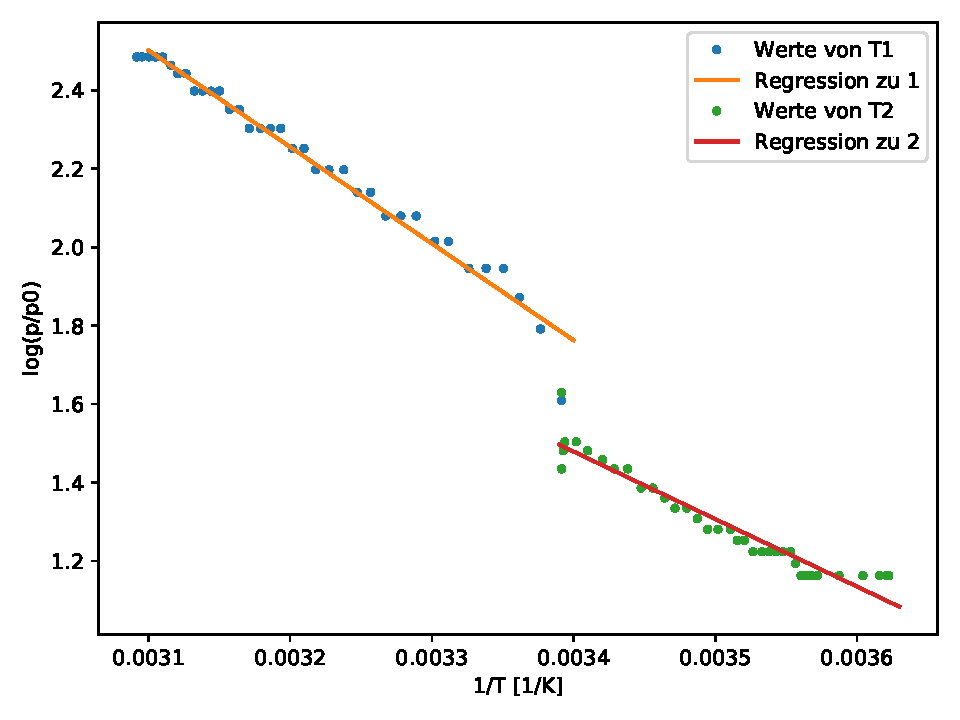
\includegraphics[width=0.7\textwidth]{build/plot2.pdf}
    \caption{Die Messwerte inklusive der Fit-Funktion.}
    \label{img:plot1}
\end{figure}

\noindent
Einsetzen der Fit-Funktionen in \refeq{eqn:ohnedp} führt zu:
\begin{equation}
    L(T)=\left( \frac{\symup{R} \cdot T}{2} \pm\sqrt{\frac{\symup{R}^2\cdot T^2}{4}-Ap} \right)\frac{3a\cdot T^3+2b\cdot T^2 + c\cdot T}{a\cdot T^3+b\cdot T^2 + c\cdot T+d}
    \label{eqn:mitdp}
\end{equation}
Das $\pm$ führt zu zwei Funktionen für die Verdampfungswärme. Durch einsetzen von beliebigen Zahlen zeigt sich, dass die Funktion
für das Minus \ref{img:minus} eine positive Steigung liefert und zusätzlich noch sehr kleine Werte. Aus diesen Gründen bietet sie keine vernünftige Lösung für $L$.\\
Die Funktion \ref{img:plus} für das Plus hingegen, liefert eine streng monoton fallende Funktion für $L$.
Dies ergibt auch Sinn, da die Verdampfungswäme immer weiter abnehmen sollte, je näher die eingesetzten Temperaturen der kritischen Temperatur kommen, bei der $L=0$ gilt.\\
Die nachfolgende Tabelle \ref{tab:Lvergleich} zeigt Theoriewerte für $L$ bei bestimmten Temperaturen und die dazu korrespondierenden Werte der zuvor gewählten Fit-Funktion.

\begin{table}[H]
    \centering
    %\caption{Die Messwerte}
    \begin{tabular}{ S [table-format=3.1] S [table-format=5.0] S [table-format=5.3] S [table-format=2.1]}
        \toprule
        {$T \mathbin{\scalebox{1.5} /} \si{\kelvin}$} & {$L_\text{Theorie} \mathbin{\scalebox{1.5} /} \si{\joule\per\mole}$}& {$L_\text{Fit$_+$} \mathbin{\scalebox{1.5} /} \si{\joule\per\mole}$}& {$Abweichung \mathbin{\scalebox{1.5} /} \si{\percent}$}\\
        \midrule
        393.1 & 39684 & 71630.765 & 80.5\\
        413.1 & 38643 & 50767.536 & 31.4\\
        433.1 & 37518 & 44745.589 & 19.3\\
        453.1 & 36304 & 41103.275 & 13.2\\
        473.1 & 34962 & 37865.484 & 8.3 \\
        \bottomrule
    \end{tabular}
\caption{Eine Tabelle, welche die Temperatur und ihre korrespondierenden Fit- und Theorie-Werte \protect \cite{Chemie-Schule.de-Verdampfungswärme} für $L$ zeigt. Außerdem ist die prozentuale Abweichung der $L$ Werte voneinander enthalten.}
\label{tab:Lvergleich}
\end{table}

\subsubsection{Plots der Funktionen der Verdampfungswärme}

Die folgenden Abbildungen zeigen die beiden gefundenen Funktionen \refeq{eqn:mitdp}.\\
Dabei wird die Dampfdruckwärme gegen die Temperatur abgetragen. Der erste Plot bildet dabei die Theoriewerte \ref{tab:Lvergleich}
und die Funktion $L_+(T)$ ab.\\
Es zeigt sich, dass die Funktion für steigende Temperaturen den Theoriewerten annähert.\\\\
\noindent
Die zweite Abbildung zeigt nur exemplarisch $L_-(T)$, um zu ersichtlich zu machen, dass die Werte der Funktion
mit dem erwarteten Ergebnis für $L$ nicht kompatibel sind.
\FloatBarrier
\begin{figure}[H]
    \centering
    \includegraphics[width=0.7\textwidth]{build/plot3+.pdf}
    \caption{Ein Plot der Funktion $L_+(T)$ und der Theoriewerte \protect \cite{Chemie-Schule.de-Verdampfungswärme}.}
    \label{img:plus}
\end{figure}



\begin{figure}[H]
    \centering
    \includegraphics[width=0.7\textwidth]{build/plot3-.pdf}
    \caption{Ein Plot der Funktion $L_-(T)$.}
    \label{img:minus}
\end{figure}

\FloatBarrier







\subsubsection{Die Messwerte bis 15 Bar}
Dies ist die Tabelle, der im zweiten Versuchsteil aufgenommenen Messwerte. 
Sie zeigt die gemessenen Drücke, so wie die gemessenen Temperaturen in Bar und Kelvin.
\begin{table}[H]
    \centering
    %\caption{Die Messwerte}
    \begin{tabular}{ S [table-format=3.0] S [table-format=3.1] S [table-format=3.1]}
        \toprule
        {$P \mathbin{/} \si{\bar}$} & {$T \mathbin{/} \si{\celsius}$} & {$T \mathbin{/} \si{\kelvin}$}\\
        \midrule
        1 & 118.0 & 391.1\\
        2 & 129.5 & 402.6\\
        3 & 141.0 & 414.1\\
        4 & 150.0 & 423.1\\
        5 & 157.0 & 430.1\\
        6 & 163.5 & 436.6\\
        7 & 168.0 & 441.1\\
        8 & 172.5 & 445.6\\
        9 & 177.0 & 450.1\\
        10 & 181.5 & 454.6\\
        11 & 185.5 & 458.6\\
        12 & 189.0 & 462.1\\
        13 & 192.0 & 465.1\\
        14 & 195.0 & 468.1\\
        15 & 198.5 & 471.6\\
        \bottomrule
    \end{tabular}
\caption{Eine Tabelle der Messwerte bis $\SI{15}{\bar}$.%wobei die Temperaturen mit einem Fehler von  $\increment T = \SI{0.1}{\celsius}$ behaftet sind.
}
\label{tab:messung2}
\end{table}


